%% V1.0
%% by Gabriel Garcia, gabrcg@gmail.com
%% This is a template for Udacity projects using IEEEtran.cls

%% Be Udacious!

\documentclass[10pt,journal,compsoc]{IEEEtran}

\usepackage[pdftex]{graphicx}    
\usepackage{cite}
\hyphenation{op-tical net-works semi-conduc-tor}


\begin{document}

\title{Exploring Weather Trends}

\author{Raunak Tripathi}

\markboth{Weather Trends Project, Data Analyst Nanodegree Program, Udacity}%
{}
\IEEEtitleabstractindextext{%

\begin{abstract}
Comma Seperated Value Files (CSV) were extracted from the udacity's portal with the help of the syntax Structured Query Language(SQL). Database was accessed from the udacity’s native workspace, downloaded in the form of CSV files which included the average temperature of the various cities and the global average temperature. Close examination of the data showed that the Global average temperature is rising exponentially and the comparison between cities were demonstrated with the help of line chart.
\end{abstract}

\begin{IEEEkeywords}
Python, SQL, Excel, Spyder (Python3), LaTEX for report generation, Udacity.
\end{IEEEkeywords}}

\maketitle
\IEEEdisplaynontitleabstractindextext
\IEEEpeerreviewmaketitle
\section{Introduction}
\label{sec:introduction}

\IEEEPARstart{C}{urrent} predictions of climate change may significantly underestimate the speed and severity of global warming. Many changes have been unprecedented over the years and continuing to an exponential extent. In this report we will analyze the database obtained from the udacity's workspace. We will also learn about working with tables and plotting a Moving Average Line chart using tools such as SQL and Python. 

Comparing London's and Dublin's average temperature with the Global average temperature, sounds fun, lets get on with it.


\subsection{Methods}
Tools such as SQL and Python3 were used to export the files to CSV and to analyze the data using Python library modules such as matplotpy and pandas whose main job is to make a fast and flexible database. Python provides an upper hand over excel because because of its ease and user-friendly. Few lines of code and plotting a graph is done without creating multiple duplicates of the database.

\subsubsection{SQL}
The CSV fies were extracted using the Udacity's native SQL Workspace:


$SELECT * \hspace{0.15cm} 
FROM \hspace{0.15cm} city\_data ;
$\\

Joining and creating a columns \\
$ALTER \hspace{0.15cm} TABLE \\ global\_data \hspace{0.15cm} RENAME \hspace{0.15cm} COLUMN \\ avg\_temp \hspace{0.15cm} to \hspace{0.15cm} global\_avg\_temp;$
\\

$ALTER\hspace{0.15cm} TABLE \\ city\_data\hspace{0.15cm} RENAME\hspace{0.15cm} COLUMN \\avg\_temp\hspace{0.15cm} to \hspace{0.15cm}london\_avg\_temp;$
\\

$ALTER \hspace{0.15cm} TABLE \\ city\_data\hspace{0.15cm} ADD\hspace{0.15cm} COLUMN \\dublin\_avg\_temp;$ \\


Now creating a inner join such that the created table can be used for plotting Moving Average line chart.

$SELECT \hspace{0.15cm} global\_data.year,\\ global\_data.global\_avg\_temp,\hspace{0.15cm}london\_avg\_temp
\\FROM \hspace{0.15cm}global\_data \hspace{0.15cm}INNER\hspace{0.15cm} JOIN\\ city\_data\hspace{0.15cm} ON \hspace{0.15cm}global\_data.year\hspace{0.15cm}=\hspace{0.15cm}city\_data.year
\\WHERE \hspace{0.15cm}city \hspace{0.15cm}like\hspace{0.15cm} 'London';
$
\\ \\ Exporting file to CSV.


\subsubsection{Python}
With the help of this powerful tool, I was able to accomplish the task of plotting the line chart using pandas for correlation of data from the table and and declaring a function such that different moving averages can be calculated with ease. dropna() from Pandas module is used to reduce the noise from the CSV file.

output temperature = input temperature. function(window = temperature).mean().dropna()

Moving Average are calculated only after cleaning the CSV files from error to avoid sudden fluctuations in the line chart. Thus plotting the graph will help us in giving a deep understanding and also a visual interpretation is always better than its counterpart.

So, Code for moving average:

$average\_span = 7$ \\
$moving\_avg = MeanFunction(average\_span, temp)$\\
$plt.plot(moving\_avg['year'],moving\_avg['london\_avg\_temp'], label\hspace{0.1cm}=\hspace{0.1cm}'London')$ \\
$plt.plot(moving\_avg['year'], moving\_avg['dublin\_avg\_temp'], label\hspace{0.1cm}='Dublin')$\\
$plt.plot(moving\_avg['year'], moving\_avg['global\_avg\_temp'], label\hspace{0.1cm}='Global')$

Here we have taken moving average as seven years because it gives us a wider range from which various comparisons can be made.

\subsection{Line Charts}
Using the matplotlib module of Python3, the line charts were plotted using
Spyder (Python 3) Environment provided by Anaconda Navigator. Spyder was extremely easier tool to plot graph for data analysis purpose rather than using MS Excel because it is redundant free tool. It create multiple layers of file edits rather than creating multiple files in different locations.

\begin{figure}[thpb]
      \centering
      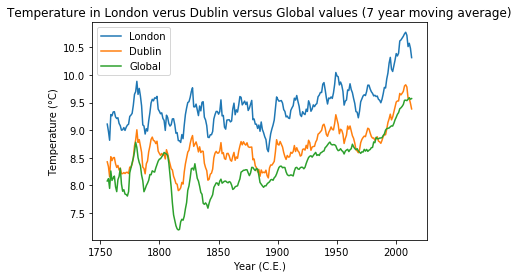
\includegraphics[width=\linewidth]{7years}
      \caption{7 years moving Average of London's versus Dublin's versus global average temperature}
      \label{fig: 7 years moving average of London's versus Dublin's versus global average temperature }
\end{figure}

Where the global Average temperature is in green color, London's average temperature is in Blue color and Dublin's average temperature is in Orange color.

It is clearly seen that the average temperature have been rising ever since the temperature were being recorded. Global warming to be blamed on this part. SO, I took a 7 year moving Average because it provided a better understanding of the line chart and gave wide range of values where the comparison can be made.

\section{Why python for plotting}
Excel has view limitations which python  can always beat. And i didn't get the idea of plotting a moving average graph in excel so, i learned more about python and ended up learning some cool modules like matplotpy and pandas and integrated that into the project. This tool provides a better understanding on Visual level. 

\begin{figure}[thpb]
      \centering
      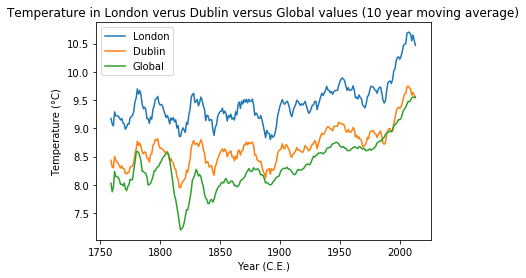
\includegraphics[width=\linewidth]{10years}
      \caption{10 years moving Average of London's versus Dublin's versus global average temperature}
      \label{fig: 10 years moving average of London's versus Dublin's versus global average temperature}
\end{figure}

\begin{itemize}
\item Here we can see that London's temperature and Dublin's temperature have increased by almost 1.5 degree Celsius within a span of 200 years. So, global warming has resulted in these cities getting warmer by the day. Global average temperature is also seen to rise with the passing years.

\item It is also seen that the with the increase in the average global temperature, London's and Dublin's temperature is also increasing. 

\item The moving Average used here is not a simple moving average but an exponential one. 

\item With the change in the London's and Dublin's temperature, the global temperature graph also tends to rise and is seen consistent. By consistent, i mean the higher the global average temperatures, higher will be there chances of hotter weather, thus a steep slope will be obtained.
\end{itemize}

. \cite{lamport1994latex}

\begin{figure}[thpb]
      \centering
      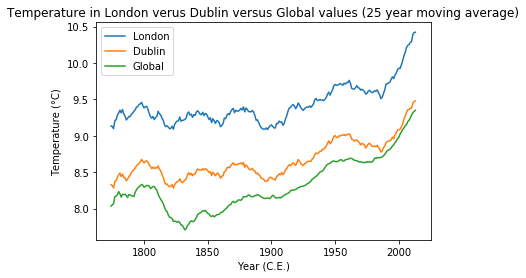
\includegraphics[width=\linewidth]{25years}
      \caption{25 years moving Average of London's versus Dublin's versus global average temperature}
      \label{fig: 25 years moving average of London's versus Dublin's versus global average temperature}
\end{figure}

\begin{figure}[thpb]
      \centering
      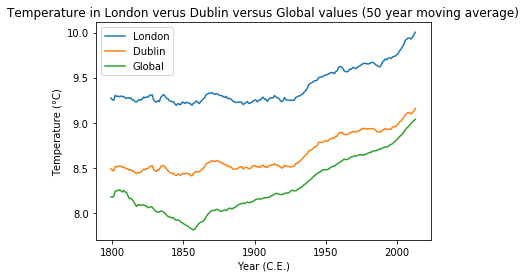
\includegraphics[width=\linewidth]{50years}
      \caption{50 years moving Average of London's versus Dublin's versus global average temperature}
      \label{fig: 50 years moving average of London's versus Dublin's versus global average temperature}
\end{figure}


\section{Working Environment}
\begin{figure}[thpb]
      \centering
      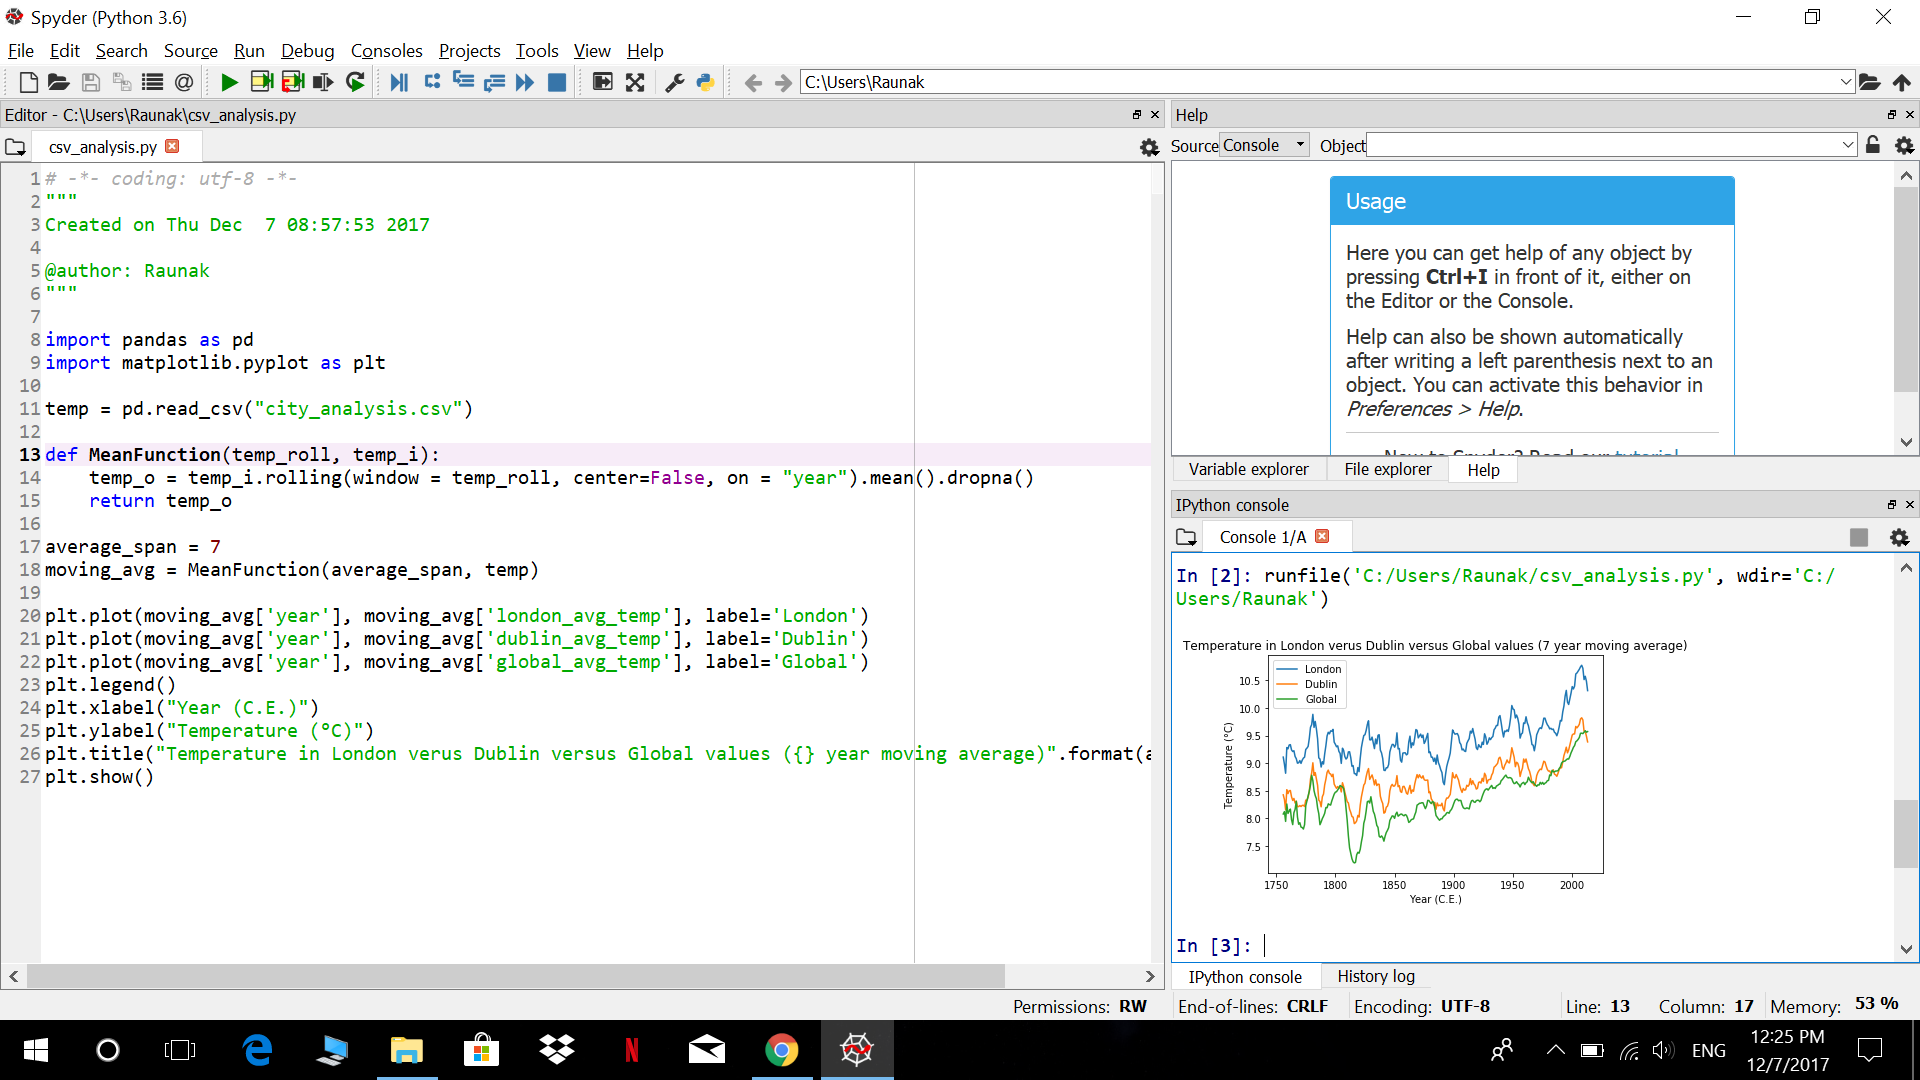
\includegraphics[width=\linewidth]{Spyder}
      \caption{Working on Spyder (Python 3.0)}
      \label{fig: Working with Spyder}
\end{figure}

\section{Discussion}
The overall trends tends to give us an idea that global warming a very serious issue and it should be taken care of.
\begin{itemize}
\item  The trends from 1950-present has seen drastic change in terms of global average temperature as well as London's and Dublin's average temperature.
\item The world is getting hotter place to live in. 
\item The temperature gives us an idea that these figure will increase exponentially until several strict measures are not taken into account. \item The trend has been consistently increasing with each passing decade and will increase or the climate change will soon plunder the planet
\end{itemize}

\bibliography{bib}
\bibliographystyle{ieeetr}
\end{document}